\documentclass[10pt]{article}

\usepackage{lipsum}
\usepackage{url}
\usepackage{float}
\usepackage{amsmath}
\usepackage{enumitem}
\usepackage{graphicx}
\usepackage{caption}
\usepackage{subcaption}
\usepackage{rotating}
\usepackage{geometry}
\usepackage{listings}
\usepackage{hyperref}
\usepackage[T1]{fontenc}
\usepackage[numbered]{matlab-prettifier}

\newcommand{\documentTitle}{Lab 2 - Signal Sources and Sinks}
\newcommand{\documentAuthor}{Andrew Pham, Aneel Damaraju}
\newcommand{\courseTitle}{ELEC 240}
\newcommand{\testDate}{September 11, 2018}
\newcommand{\reportDate}{September 18, 2018}

\geometry{margin=1in}
\lstset{
    tabsize=4,
    basicstyle={\ttfamily},
    captionpos=b,
    belowskip=1em,
    aboveskip=1em,
    numbers=left,
	escapechar=\@,
}

\title{
    \textbf{\courseTitle} \\
    \textbf{\documentTitle} \\
    \bigskip
    \textbf{\large{Test performed: \testDate}} \\
    \textbf{\large{Report submitted: \reportDate}} \\
    \bigskip
    \bigskip
}
\author{\documentAuthor}
\date{}

\begin{document}

\maketitle

\newpage

\section{Objective}

In this lab, we explored how to detect and change signals through the use of electroacoustic transducers. In the first section, we observed the various properties of a signal such as its frequency and amplitude through a speaker and calculated how measuring this signal with the speaker affects the circuit. In the second section, we now produced signals through various methods like our vocal cords and the lab PC and viewed these signal properties on the oscilloscope. Finally, in section three, we independently viewed the signal properties of a photodiode and a light-emitting diode, then combined the two to view how a light-emitting diode can send signals to a photoresistor to achieve optoelectronic communication. 

\medskip

%\textit{Note (To be deleted): Think of this test report as a document with your peers as your readers. This means you can assume a similar knowledge background as you. Your readers should be able to easily understand what is going on, and also be able to repeat your lab results based on your document and all references you cite.}



%\textit{For the Objective section, identify the test you performed and its objectives. The objectives of the test are important to state because they are usually analyzed in the conclusion to determine whether the test succeeded.}

\section{Materials and Pre-Lab Work}

\begin{itemize}
	\item Virtual Bench (Software, Oscilloscope, Function Generator, DC Power Supply)
	\item BNC Male to Clips cord
	\item Oscilloscope Probe
	\item Speaker
	\item Breadboard
	\item Microphone
	\item 2 10 cm length wires (with 6 mm stripped on each end)
	\item Lab PC with associated sound files and sound card cable
	\item Photodiode 
	\item Red LED
	\item BNC Banana Adapter
	\item Digital Multimeter
	\item 220 Ohm Resistor
\end{itemize}

\medskip

%\textit{Note (To be deleted): Provide a bullet point list of components, software tools, and hardware (such as the NI VirtualBench or DMM) used during the lab}

\section{Test Description}

\subsection{Electroacoustic Transducers I}
We began by creating a 1kHz sine wave, connecting this signal to a speaker, and listening to the signal in audio form. We then varied the parameters of the input signal to listen to the effects on the output signal. Then using these measurements, we found the Thevenin voltage, and used this value to attempt to find the maximum power transfer.

\subsection{Electroacoustic Transducers II}
This time, we varied the input of the oscilloscope by attaching it to a microphone. After making various sounds into the microphone and visualizing the signals, we attempted to qualitatively analyze the signals created by vowels sounds created by humans as well as a virtual piano. After this, we attempted to analyze various given audio signals through the use of a speaker and the oscilloscope attached to the sound card cable of the computer playing the sounds.

\subsection{Optoelectrical Signal Sources and Sinks}
We created a simple circuit connecting a photodiode to the oscilloscope and observed the AC and DC signals created by this circuit before and after covering the diode with a hand. After this a LED was connected to the DC power supply. and qualitative observations were recorded while varying the amplitude and frequency of the incoming voltage. Then the optical source and sink were combined, and the measurement across the photodiode was read as it received signals from blinking LED.

\medskip

%\textit{Note (To be deleted): This section provides a summary of the test your team performed. Give enough information so readers can understand what you did, but do not go into the details of every step.}

\section{Pre-Lab Calculations and Schematics}

\begin{center}
	\begin{figure} [H]
		\centering
		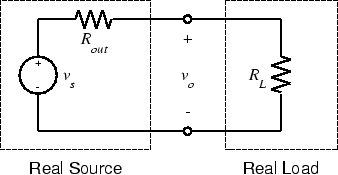
\includegraphics[scale=0.5]{images/prelab.png}
		\caption{Given Pre-lab Schematic to understand load resistances for the purpose of Thevenin Voltages}
	\end{figure}
\end{center}
No pre-lab calculations were needed, but understanding of \textit{Figure 1} was important. This figure highlights the importance of not discrediting the resistance of the  measuring instrument. This is important in Experiment 2.1 for the understanding of Thevenin equivalents.

We began setting up for the first part of the lab by gathering a microphone and the necessary cables from the supply room (listed above in the materials section) and by powering up the lab PC and starting up Virtual Bench. 

\medskip

%\textit{Note (To be deleted): Include the homework pre-calculations and schematics that serve as the initial setup for the test. Briefly explain the importance of each item you include. You may want to number your equations/figures so you can refer to them in later sections. Including photos of handwritten work is okay.}

\section{Results and Discussion}

\subsection{Experiment 2.1: Electrostatic Transducers I}
\subsubsection{Part A}
\begin{itemize}
	\item After connecting the 1kHz sine wave to the speaker, we heard a constant-pitch sound from the speaker.
	\item Measuring the voltage signal with an oscilliscope yielded a peak-to-peak measurement of 164.6 mV. This is because the speaker acts as a resistor, causing a proportional drop in voltage amplitude of the input signal. 
	\item We then varied the parameters of the input signal. Increasing the frequency increases the pitch of the tone. Increasing the amplitude of the tone increases the volume of the tone. By changing the sinusoid to a square wave, the sound becomes a flatter, more piercing tone. 
\end{itemize}

\subsubsection{Part B: Thevenin Equivalent and Maximum Power Transfer}
By analyzing the in \textit{Fig. 1}, we find that the Thevenin voltage is 5V. We then measured the voltage drops across various resistors when connected in series with the 5V DC power supply. We obtained the following voltage drops:
\begin{itemize}
	\item \textbf{20 Ohms}: 1.453 V
	\item \textbf{30 Ohms}: 1.891 V
	\item \textbf{50 Ohms}: 2.515 V
	\item \textbf{100 Ohms}: 3.31 V
\end{itemize} 

We then calculated the $R_{OUT}$ (based on \textit{Fig.1}) for each of the resistors and obtained the following values for $R_{OUT}$ for each resistor (in bold):
\begin{itemize}
	\item \textbf{20 Ohms}: 48.823 Ohms
	\item \textbf{30 Ohms}: 49.323 Ohms
	\item \textbf{50 Ohms}: 49.404 Ohms
	\item \textbf{100 Ohms}: 51.0574 Ohms
\end{itemize} 

As we can see from our calculated $R_{OUT}$ values for each resistor, the $R_{OUT}$ of the circuit is approximately 50 Ohms. Therefore, the Thevenin resistance does not change. 

We then calculated power using the formula $P_{avg}= 0.5 * {V_M}^2 * R_L$ where $V_M$ is the maximum amplitude of the voltage drop across the load resistance $R_L$. We obtained the following power values for each of the resistors (in bold):
\begin{itemize}
	\item \textbf{20 Ohms}: 125.81 W
	\item \textbf{30 Ohms}: 144.99 W
	\item \textbf{50 Ohms}: 154.38 W
	\item \textbf{100 Ohms}: 142.81 W
\end{itemize} 

\textit{Fig. 2} depicts the Power vs $R_L$ relationship:
\begin{center}
	\begin{figure} [H]
		\centering
		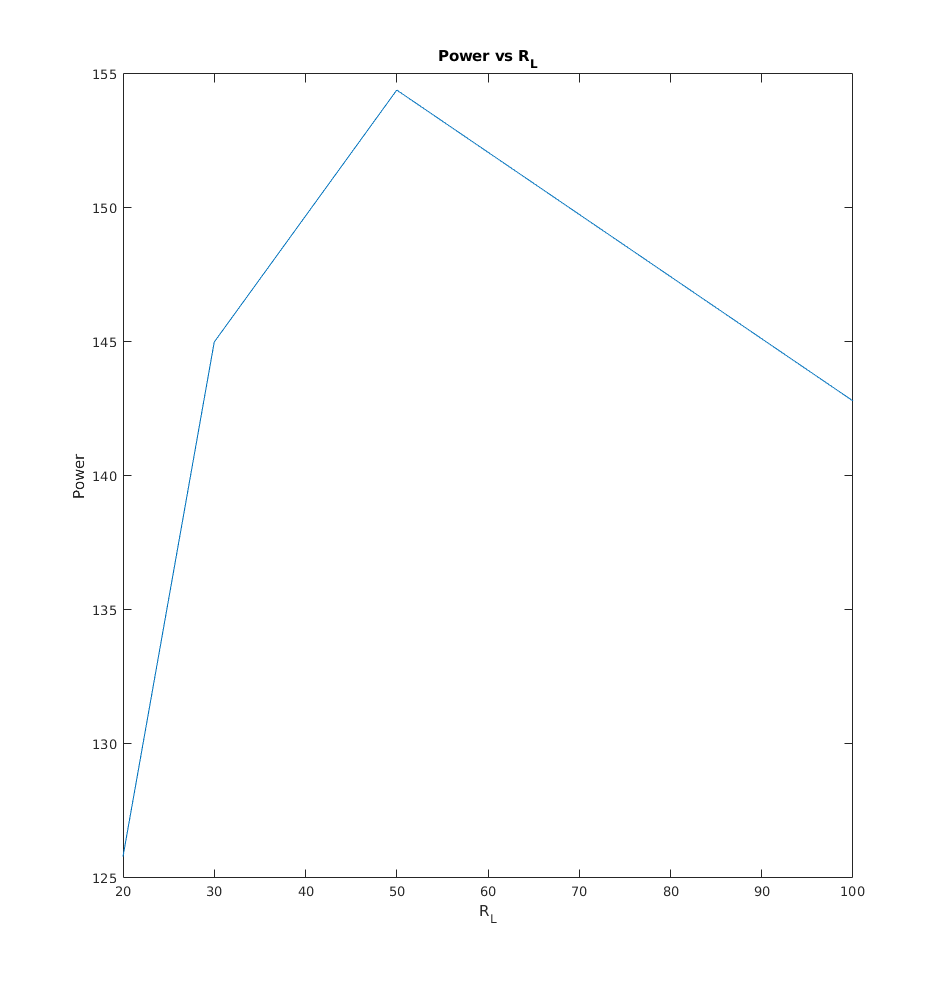
\includegraphics[scale=0.4]{images/powerplot.png}
		\caption{Power vs $R_L$ relationship}
	\end{figure}
\end{center}



We can see from our calculations that these measurements satisfy the Maximum Power Transfer Theorem, which states that the maximum power is delivered to the load when the load resistance is equal to the Thevenin resistance of the source ($R_L = R_{OUT} = 50$ Ohms)

\subsection{Experiment 2.2: Electrostatic Transducers II}
\subsubsection{Part A: Microphone}
\begin{itemize}
	\item We connected the connected the microphone to the oscilloscope by first connecting the microphone to the J1-4 port on the breadboard, then connecting the J1-4 to the J1-1 port, then connecting the oscilloscope to that J1-1 port. We then whistled into the microphone. We adjusted the trigger to 5 mV above the origin. By doing so, we were able to essentially "freeze" the sinusoid so that we could better view its properties. 
	\item We then sang the 5 vowel sounds into the microphone. We found that the vowel A was the most sinusoid-like. \textit{Fig. 3} is the sound of an "A" in comparison to the sound of "O" in \textit{Fig. 4}. 
\end{itemize}

\begin{enumerate}
	\item  We then played a perfect "A" tone off a smartphone speaker into the microphone. The resulting signal was a near-perfect sine wave with a frequency of 440 Hz as opposed to the vocally generated "A" signal in \textit{Fig. 3} with a frequency of 623 Hz. The discrepancy in frequency arose from the fact that a human can sing an "A" sound at a different pitch than the offical "A". 
\end{enumerate}

\begin{center}
	\begin{figure}[H]
		\centering
		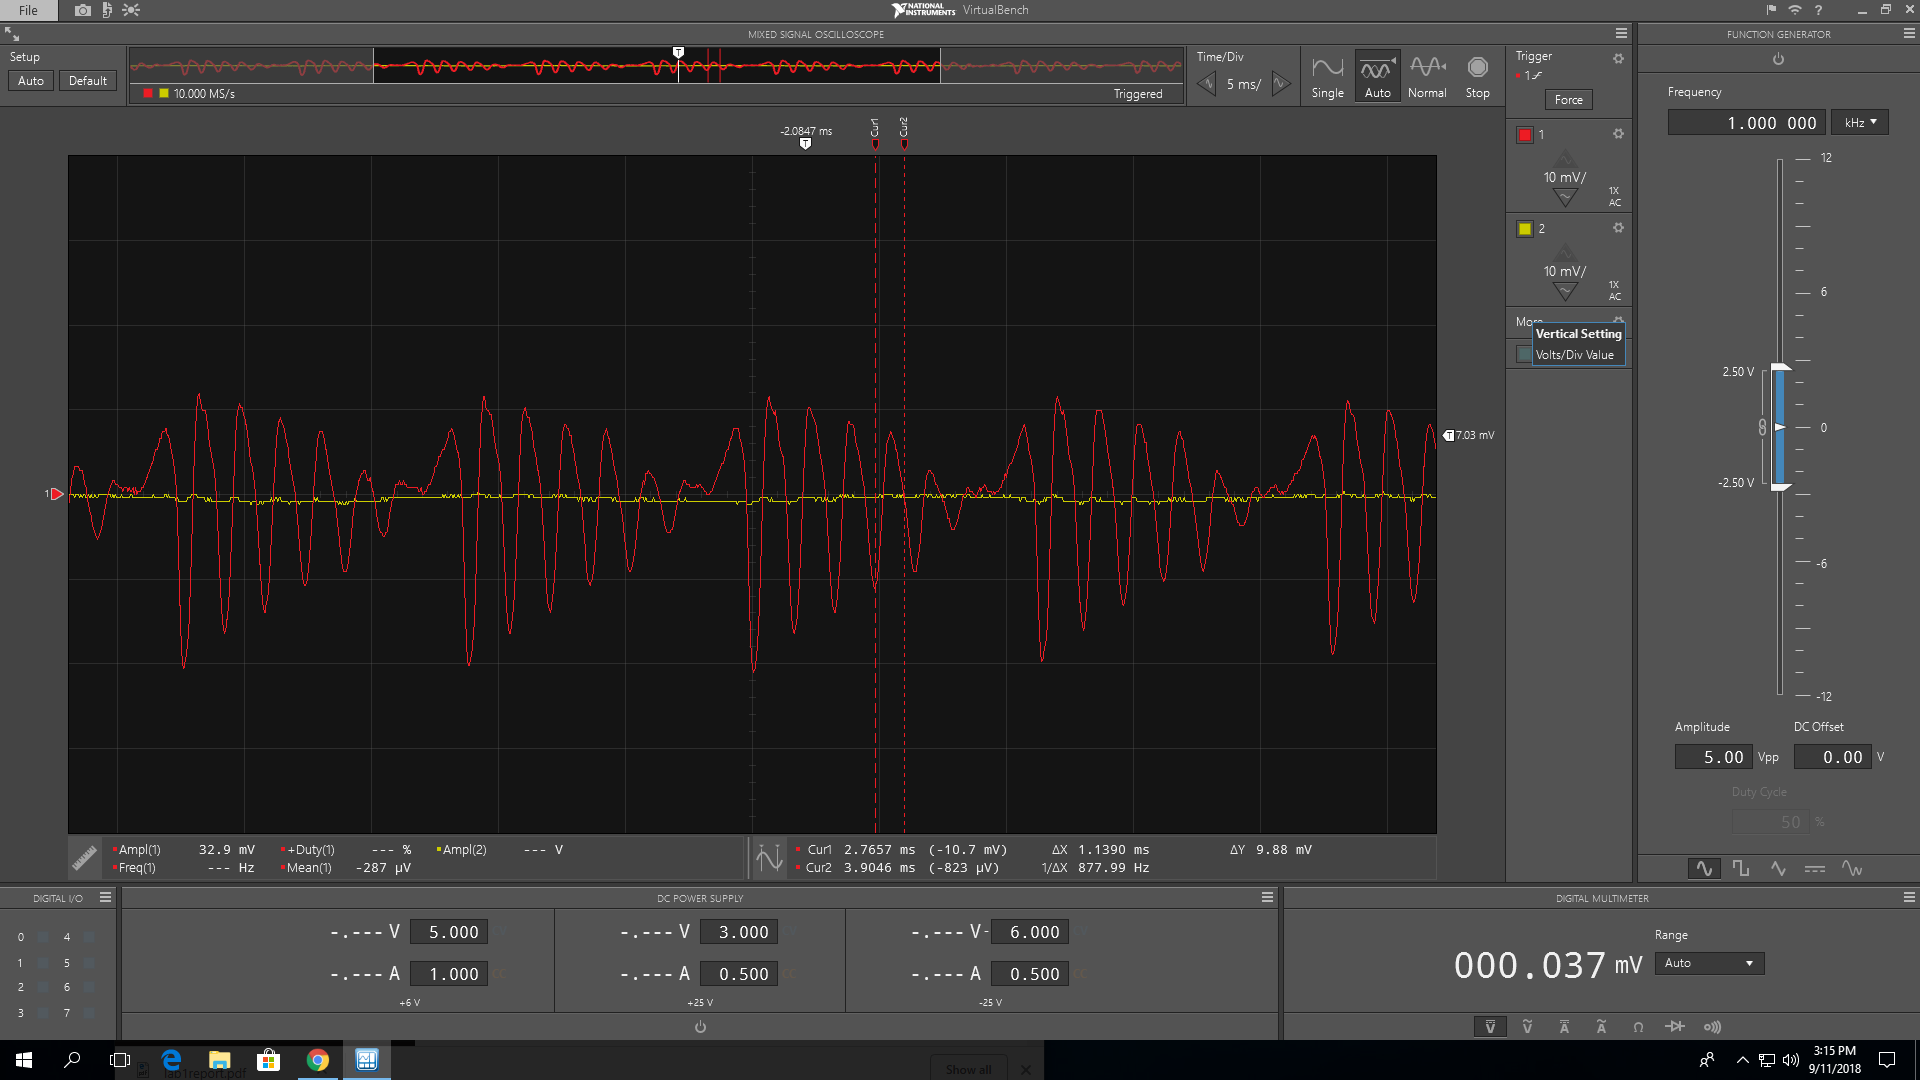
\includegraphics[scale=0.22]{images/aaa.png}
		\caption{Sine Wave of Vocally Produced Vowel "A" Sound}
	\end{figure}
	\begin{figure}[H]
		\centering
		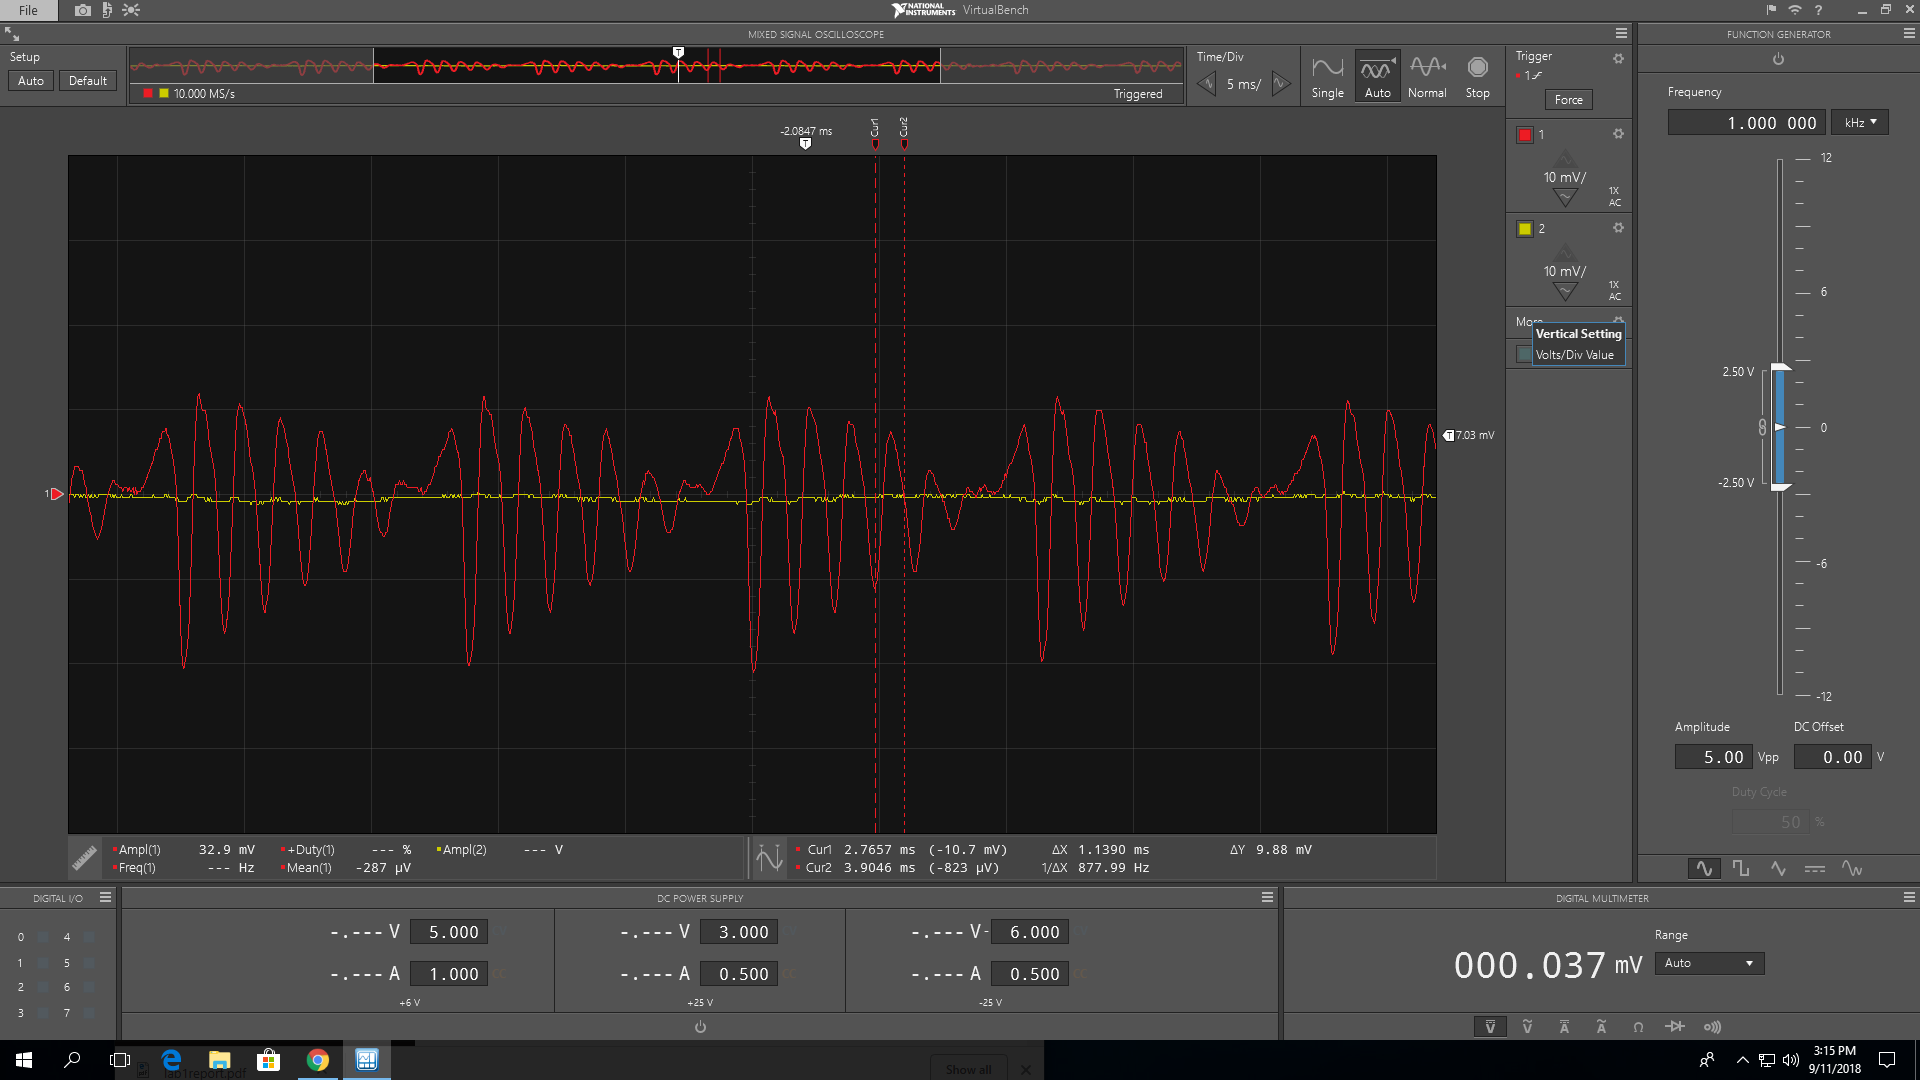
\includegraphics[scale=0.22]{images/ooo.png}
		\caption{Sine Wave of Vocally Produced "O" Sound for comparison}
	\end{figure}
\end{center}

\subsubsection{Part B: The Lab PC as a Signal Source}
In this section, we connected the Lab PC to the oscilloscope by first connecting the lab PC to the J2-1 port, connecting the J2-1 port to the J1-3 port, and then connecting the speaker to the J1-3 port. We also kept the connection between the speaker and the oscilloscope from Part A. We then played the three sound files through the speaker and observed the signals through the oscilloscope. \textit{Fig. 5} displays the oscilloscope readings of the mystery signal. 
\begin{center}
	\begin{figure} [H]
		\centering
		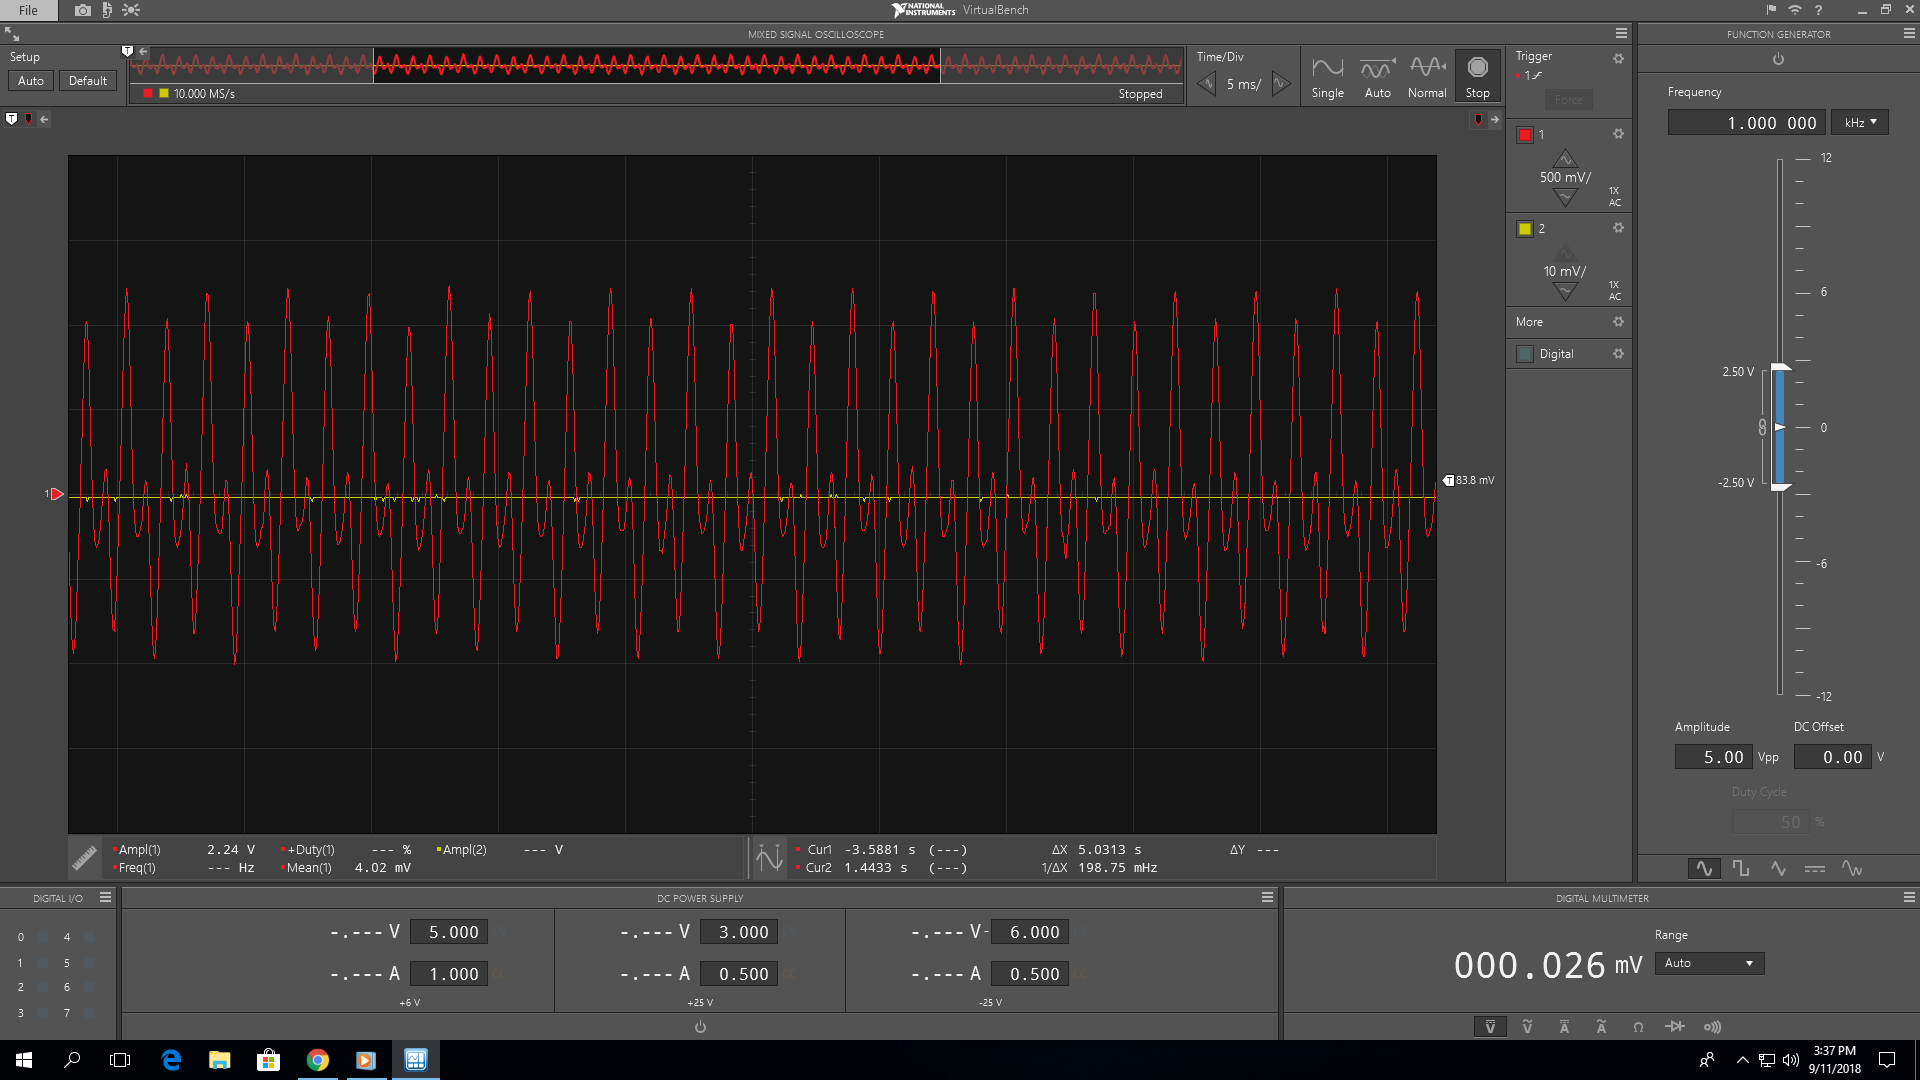
\includegraphics[scale=0.22]{images/mystery.png}
		\caption{Oscilloscope reading of the Mystery Signal}
	\end{figure}
\end{center}

The mystery tone is a Shepard tone. It is a superposition of constantly increasing sine waves (where each individual sine wave increases in frequency equivalent to one octave). The tone gives the impression of a constantly increasing pitch. 


\subsection{Experiment 2.3: Optoelectrical Signal Sources and Sinks}
\subsubsection{Part A: The PhotoDiode}
We begin this section by connecting the cathode of the photodiode to pin 14 and the anode to pin 1 (which was connected to the channel 1 of the oscilloscope). We then noted the following voltages produced by the photodiode in different environments:
\begin{itemize}
	\item Photodiode in well-lit environment: -177 mV
	\item Photodiode covered by hand: -17.8 mV
\end{itemize}

We then set the oscilloscope to measure AC signals from the photodiode. The peak-to-peak amplitude of signal was 2.88 mV and the frequency was 196.83 kHz. The waveform is sinusoidal with periodic spikes in amplitude that occur in tight clumps depicted in \textit{Fig. 6} below. 
\begin{center}
	\begin{figure} [H]
		\centering
		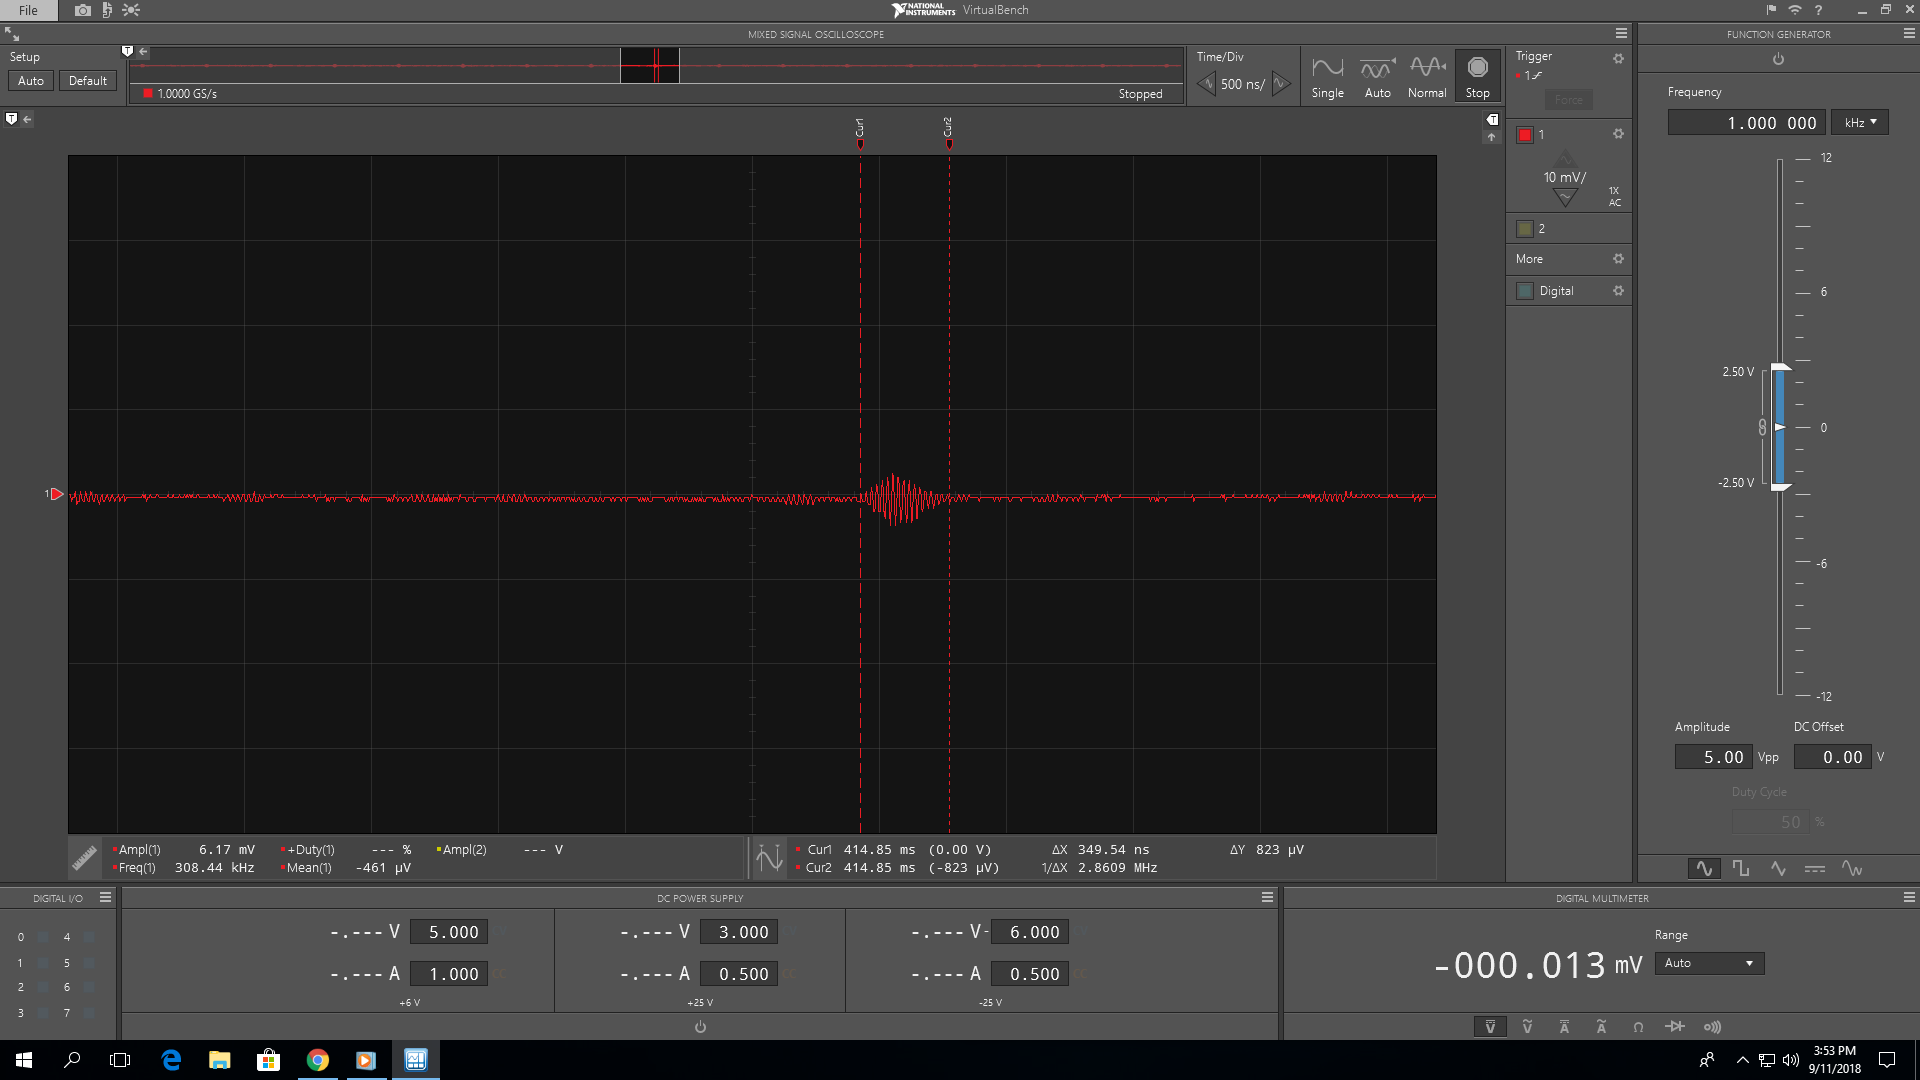
\includegraphics[scale = 0.22]{images/zoom.png}
		\caption{Oscilloscope Reading of AC signal from Photodiode}
		\label{fig:zoom}
	\end{figure}
\end{center}

\subsubsection{Part B: Light Emitting Diode}
We began by connecting the red LED in series with a 220 Ohm resistor and the VirtualBench DC power supply. We then connected a voltmeter across the leads of the LED. We then began to slowly increase the voltage of power supply. The LED visibly began to glow at 1.7 V. When the power supply set to 
\begin{itemize}
	\item 3V, the LED voltage was 1.731 V and the LED was dimly lit
	\item 4V, the LED voltage was 1.753 V and the LED was slightly brighter
	\item 5V, the LED voltage was 1.767 V and the LED glowed brightly
\end{itemize}

We then swapped the DC power supply for a 100 Hz square wave. We found that a square wave needed a peak-to-peak amplitude of 3V for the LED to appear illuminated. We then began reducing the frequency of the square wave. At 40 Hz, the LED began to flicker. This frequency is reasonably close to the industry standard of shooting films at 24 fps. We noticed the flicker at 40 Hz because we were intently focusing on a single color at a single point. When looking at an entire screen with multiple moving objects, this frame rate gives the effect of a motion blur. 

\subsubsection{Part C: Optical Communication}
We left the setup for Part B in place (though we reset the square wave back to a frequency to 100 Hz). We connected the photodiode to CH1 of the oscilloscope and then held the photodiode head right above the red LED head and shielded the components with our hand. \textit{Fig. 7} depicts the oscilloscope reading. The waveform is ....
\begin{center}
	\begin{figure} [H]
		\centering
		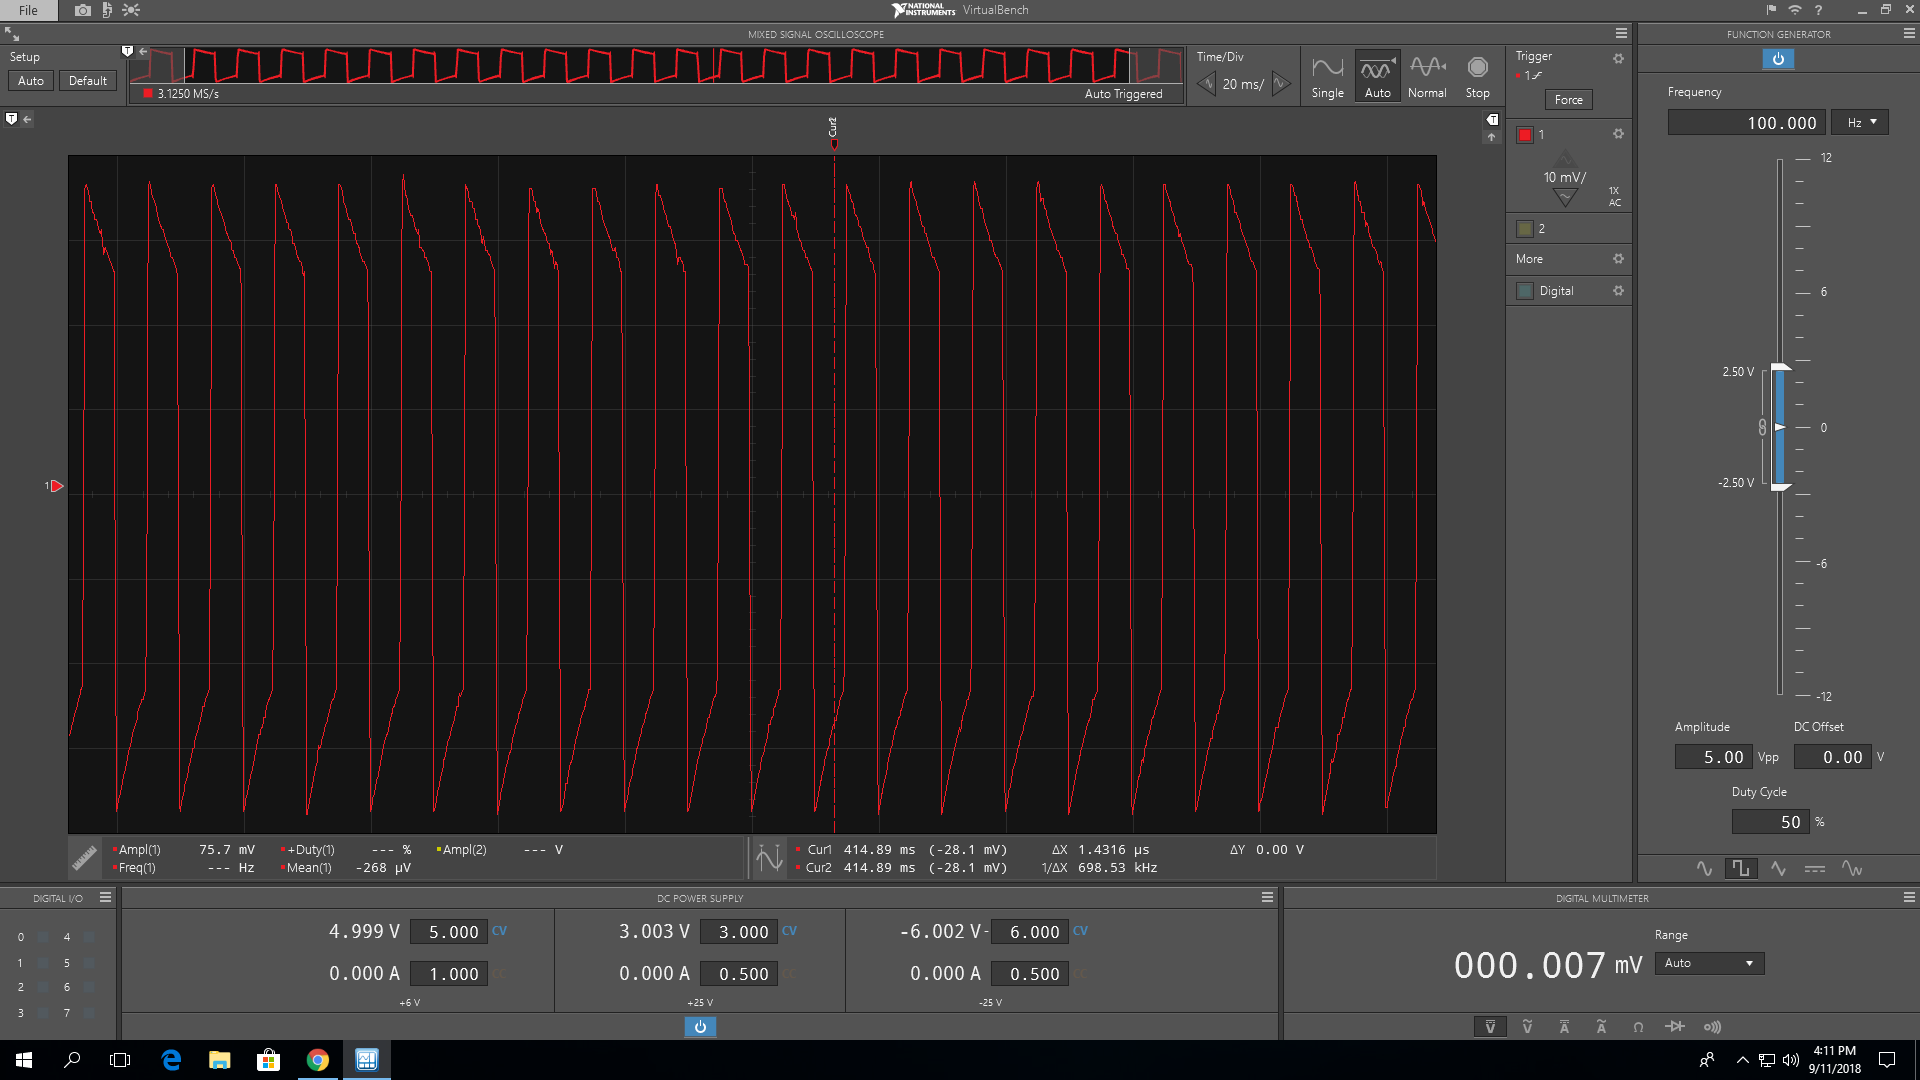
\includegraphics[scale=0.22]{images/opticalsquare.png}
		\caption{Oscilloscope reading of a photodiode voltage when exposed to an LED powered by 100 Hz square wave}
	\end{figure}
\end{center}

We then switched the square wave to a triangle wave as seen in \textit{Fig. 8}. The waveform appears to be 
\begin{center}
	\begin{figure} [H]
		\centering
		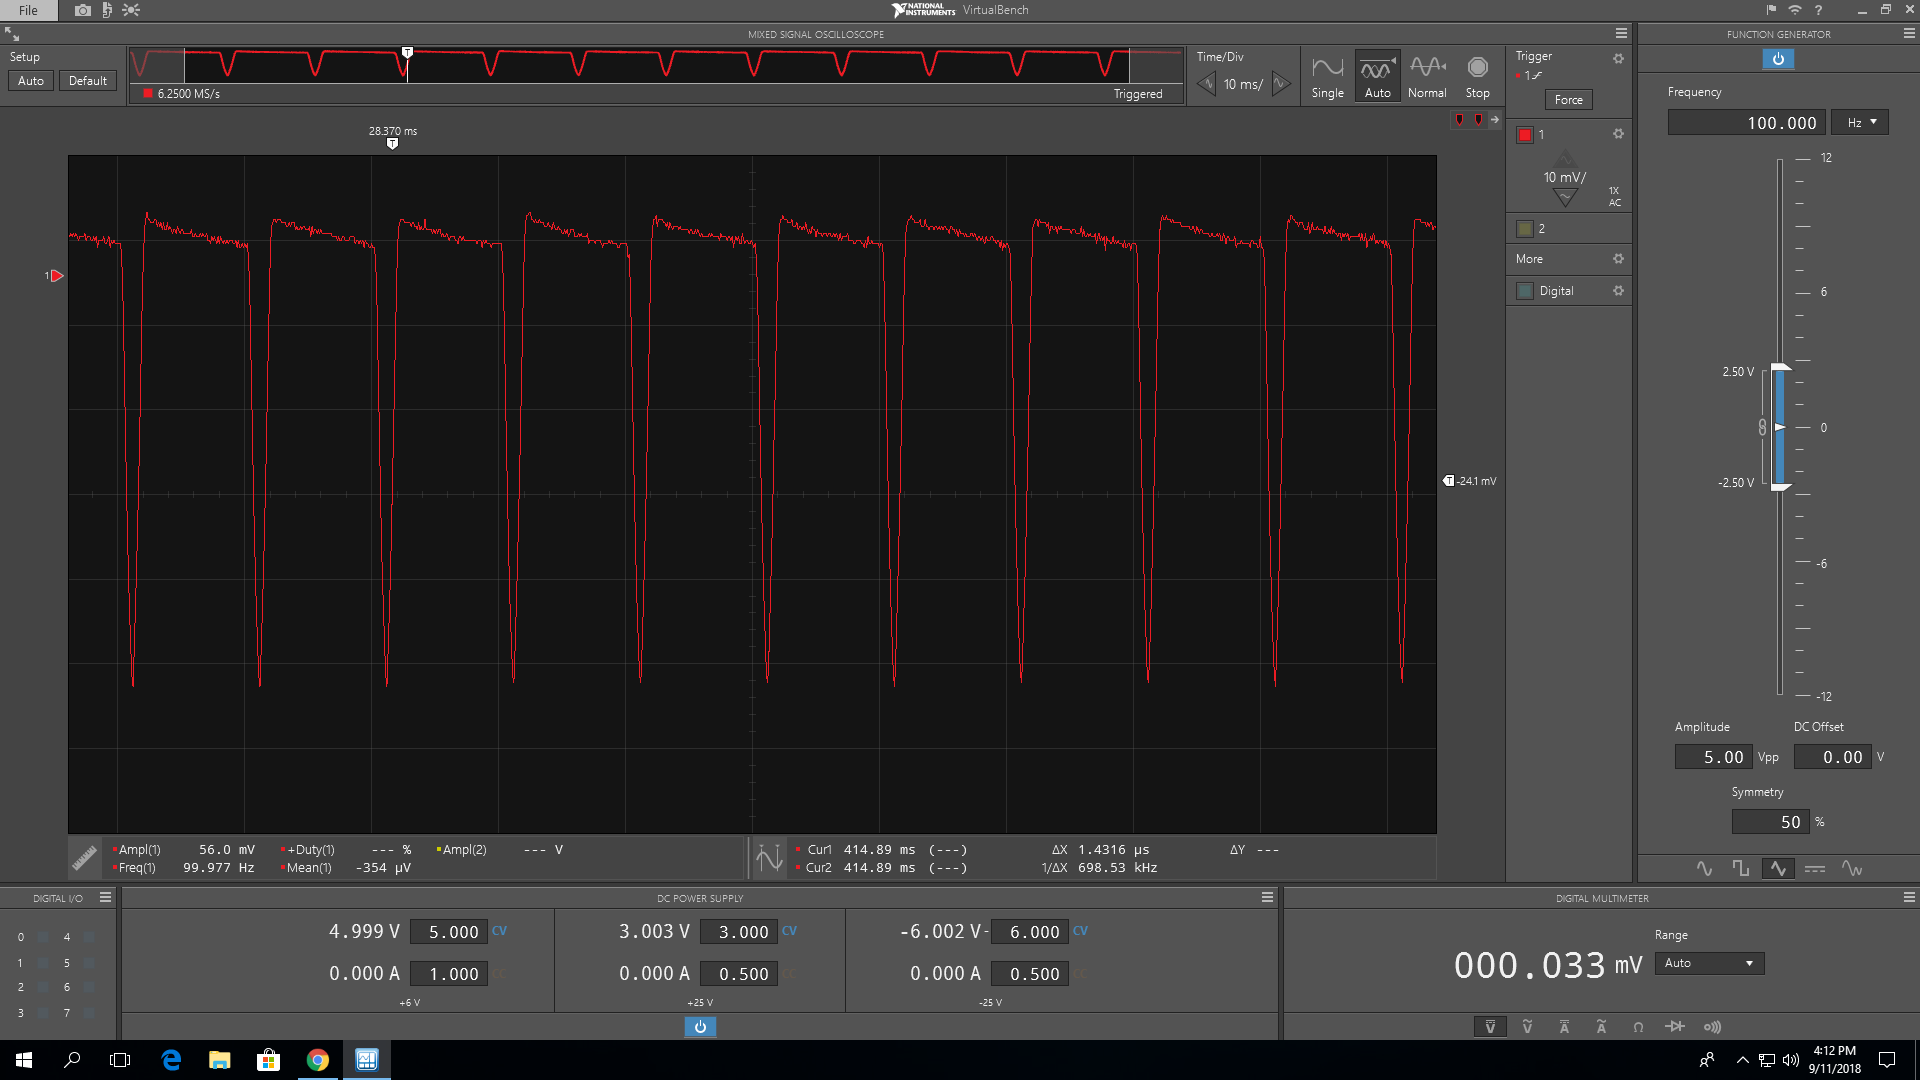
\includegraphics[scale=0.22]{images/opticaltriangle.png}
		\caption{Oscilloscope reading of a photodiode voltage when exposed to an LED powered by 100 Hz triangle wave}
	\end{figure}
\end{center}

We reset the function generator to produce a 100 Hz square wave. We found that the maximum distance that we could transmit a signal from the LED to the photodiode was 24 inches. \\
The above setup is a precursor to a basic optical communication system. However, we would also need 
\begin{itemize}
	\item some sort of tunnel so that there isn't any interference from ambient light
	\item an encoder so that we can transform data into bits and an associated decoder so that it can decode the bits into the same information
\end{itemize}
A modern problem that has been experienced by Microsoft with their intercontinental optical communication system is that pirates will occasionally steal the cable as it is being laid down. Future efforts will likely be dedicated to solving this issue. 
\medskip

%\textit{Note (To be deleted): The heart of your report is the presentation of your results and a discussion of those results. In your discussion, you should not only analyze your results, but also discuss the implications of those results.}

\section{References}

	\begin{enumerate}
		\item https://www.ece.rice.edu/~dpr2/elec240/lab1/
		https://www.youtube.com/watch?v=BzNzgsAE4F0 \textit{information on Shepard tones}
	\end{enumerate}
\medskip


\section{Conclusion}
\subsection{Experiment 2.1: Electroacoustic Transducers I}
\qquad For Part A: we found that changing the two major properties of a sine wave, the frequency and the amplitude have direct effects on the output sound as the signal travels through a speaker. Increasing the frequency increases the pitch, and increases the amplitude increases the volume.

For Part B: We found that the Thevenin Equivalent Resistance from the source does not change, which is unsurprising because it should be a constant value. We also replicated the Maximum Power Transfer figure by observing that the most power transfer occurred when $R_{OUT} = R_L$. 

\subsection{Experiment 2.2: Electroacoustic Transducers II}
For Part A: Instead of using a function generator to create an output, we used our own voices through a microphone to create signals. These signals were not as clear as the function generated signals, but it was obvious that they had the same relation to the frequency and amplitude. When this test was done for all vowels, it was clear that the "a" sound was the most sinusoidal, which makes sense when understanding why it is such a popular tuning frequency and an actual musical note. We also used the trigger function to better understand these irregular tones, as it helped to notice periodicity. There were also some interesting comparisons to be made when looking at the difference in our (poorly) sung "a" tone and the computer generated one. The computer generated tone was much more steady than the sung tone, even if it did not sound obvious it was visually obvious. 

For Part B: Like Part A was comparing sounds and created waveforms, so was this Part, except with more complex sound files. The first two files, a sine wave and a gong noise, were very straight forward, and it was clear that the gong fading was easily represented by the decaying amplitude of the sounds as seen in the images provided by the oscilloscope. The mystery signal was more interesting, after it was clear that what sounded like a chromatic scale was actually a combination of a couple of various sounds repeated over and over. When research was done into this pattern, it was discovered to be called a Shepard tone, which is a superposition of octaves at varying amplitudes that creates the feeling of each note sounding slightly different from each other.

\subsection{Experiment 2.3: Optoelectrical Signal Sources and Sinks}

For Part A: The photodiode is essentially a tiny solar cell, so it was no surprise when the change in light shining into the diode changed the output voltage. However,the output waveform in AC was a little surprising, but could have been created for a variety of reasons. The first is that the photodiode was only uncovered for a short amount of time, leading to the burst of signal. The other is that the photodiode was instantly exposed to a phone flashlight at close range, which may have caused the diode to attenuate and incorrectly output the value of the light it received.

For Part B: The LED did not light at low voltages, probably because the current flowing through the circuit was not enough to produce a visible light. However, when the light was lit, increasing the voltage provided a clear increase in brightness. The including a square wave with varying frequencies provided interesting information as well, including the threshold at which we could see the flickering of the light, 40 Hz. This value is higher than that of movies, but of course we were much closer to the source and only looking at a single changing light which could have impacted our measurements. 

For Part C: The waveform is almost what was expected for a square wave, just with a small falloff at the end of the waveform. The triangle wave was less expected, because the diode should only see part of the waveform due to the nature of the diode. The recognizable light pattern from the LED was picked up by the photodiode up to a distance of 2 feet, in optimal conditions such as behind a jacket. This technology is used in optical fibers today.

\medskip

\section{Errors}
\begin{itemize}
	\item \textit{The vocally produced "A" in Section 2.2 Part B was not a perfect sinusoid of 440 Hz}: This error occurred because 1) an "A" sound can be sung at slightly different pitches and 2) an untrained human voice cannot sing a steady note. Remedy this error by getting a trained vocalist. 
	\item \textit{Slight Discrepancies in Calculated $R_{OUT}$} For the 20 and 30 Ohm resistors, we strung 10 Ohm resistors in series, which caused the overall resistance to be slightly more than thirty. This explains why our calculated $R_{OUT}$ is slightly lower for these resistors. To remedy this, use more precise resistors. 
\end{itemize}


\medskip

%\textit{Note (To be deleted): Briefly list sources of error and discuss how to eliminate or deal with them}

\end{document}
